%------------Ejercicio 1---------------------------------------

\begin{question}
    Sean los campos $\psi (x,y) = \ln(\sqrt{x^2+y^2})$ y $\boldsymbol{F}(x,y)= \left(\psi_y(x,y), -\psi_x(x,y)\right)$
    \\y sea $C$ una curva regular, simple, y cerrada con orientación positiva contenida en el conjunto
    $A=\left\{(x,y): 1 < x^2+y^2 < 9 \right\}$. Hallar los posibles valores de la integral de $\boldsymbol{F}$ sobre $C$.
\end{question}

%------------Ejercicio 2---------------------------------------

\begin{question}
    Calcular el volumen del cilindro $x^2+y^2 \leq 9$ limitado por el plano $z=-1$ y el
    paraboloide $z=x^2+y^2$.
\end{question}

%------------Ejercicio 3---------------------------------------

\begin{question}
    Calcule el flujo del campo vectorial $\boldsymbol{F}(x,y,z)= (xz,-y^2,xz)$ a través de la superficie
    $S_1=\left\{x^2+y^2=1 \land 0\leq z \leq 3\right\}$ unión $S_2=\left\{x^2+y^2\leq 1 \land z=0\right\}$.
    Indique gráfica y analíticamente la orientación elegida.
\end{question}


%------------Ejercicio 4---------------------------------------

\begin{question}
    Sea $S$ una superficie en $\mathbb{R}^3$ que encierra un volumen $\Omega$ y sea el campo
    $\boldsymbol{F}(x,y,z)=(ax,2y,z)$ con $a \in \mathbb{R}$. Hallar $a$ tal que el flujo saliente de $\boldsymbol{F}$ a través de $S$
    sea igual al volumen de $\Omega$.
\end{question}

%------------Solucion 1---------------------------------------
\newpage
\begin{solution}

    Antes que nada, se debe determinar cuál es la expresión del campo $\boldsymbol{F}$, en $\mathbb{R}^3-\{(0,0)\}$.
    \begin{align*}
        \psi_x&=\partialx\left(\ln{\sqrt{x^2+y^2}}\right)\\
        &=\frac{1}{\sqrt{x^2+y^2}} \cdot \frac{1}{2\sqrt{x^2+y^2}} \cdot 2x^2\\
        &=\frac{x}{x^2+y^2}
    \end{align*}
    \begin{align*}
        \psi_y&=\partialy\left(\ln{\sqrt{x^2+y^2}}\right)\\
        &=\frac{1}{\sqrt{x^2+y^2}} \cdot \frac{1}{2\sqrt{x^2+y^2}} \cdot 2y^2\\
        &=\frac{y}{x^2+y^2}
    \end{align*}
    \begin{equation*}
        \therefore \boldsymbol{F}(x,y)= \left(\frac{y}{x^2+y^2}, -\frac{x}{x^2+y^2}\right)
    \end{equation*}
    Para comenzar a resolver el problema, se consideran todas las curvas $C_1$ regulares, simples y cerradas, orientadas positivamente
    y contenidas en $A$ tal que su región encerrada $D_1$, a su vez, también esté contenida en $A$. 
    \begin{center}
        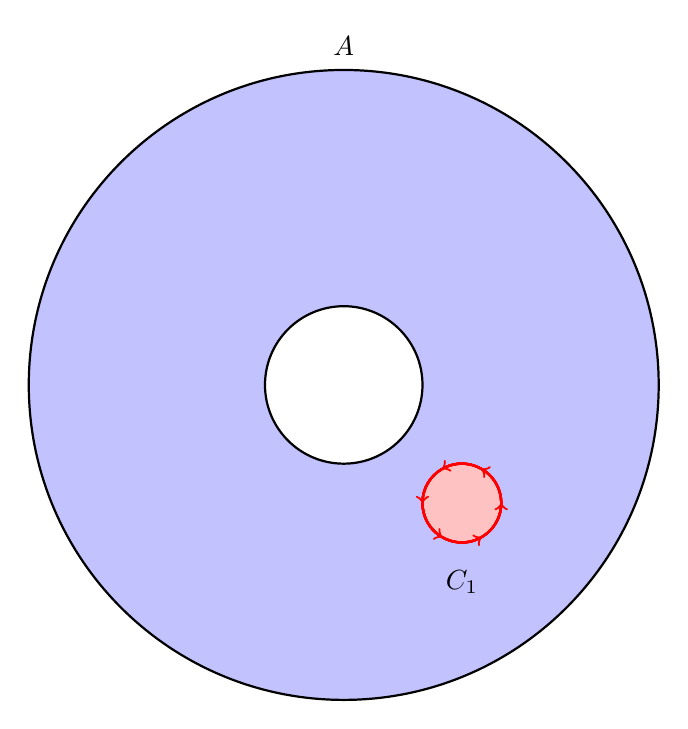
\begin{tikzpicture}
            % Define the exterior boundary
            \draw[thick, fill=blue!60!white!40] (0,0) circle (4);
        
            % Define the inner boundaries
            \draw[thick, fill=white] (0,0) circle (1);

            \draw[thick, red, fill=red!60!white!40] (1.5,-1.5) circle (0.5);
            \foreach \angle in {0, 60, 120, 180, 240, 300} {
                \draw[thick, red, ->] ({1.5+0.5*cos(\angle)}, {-1.5+0.5*sin(\angle)}) arc[start angle=\angle, end angle=\angle+360, radius=0.5];
            }

        
            % Label the regions
            \node at (0,4.3) {$A$};
            \node at (1.5,-2.5) {$C_1$};
            %\node at (0,1.4) {$C_0$};
        
        \end{tikzpicture}
    \end{center}
    En este caso, con $boldsymbol{F}$ una función de clase
    $\mathcal{C}^1$ en $A$, valen las hipótesis del teorema de Green (tanto para la curva como para el campo). Entonces:
    \begin{equation*}
        \int_{C_1}\boldsymbol{F}\cdot d\boldsymbol{s} = \iint_{D_1}\left(\grad \times \boldsymbol{F}\right)dA
    \end{equation*}
    Acto siguiente, se calcula el rotor de $\boldsymbol{F}$, para resolver la integral.
    \begin{align*}
        \grad \times \boldsymbol{F} &= \partialx\left( -\frac{x}{x^2+y^2}\right) - \partialy\left(\frac{y}{x^2+y^2}\right)\\
        &= \left(-\frac{(x^2+y^2)-2x^2}{\left(x^2+y^2\right)^2}\right) - \left(\frac{(x^2+y^2)-2y^2}{\left(x^2+y^2\right)^2}\right)\\
        &= -\left(\frac{-x^2+y^2}{\left(x^2+y^2\right)^2}+\frac{x^2-y^2}{\left(x^2+y^2\right)^2}\right)\\
        &= -\left(\frac{-x^2+y^2+x^2-y^2}{\left(x^2+y^2\right)^2}\right)\\
        \grad \times \boldsymbol{F}&= 0
    \end{align*}
    Por lo tanto, la integral del campo sobre $C_1$ resulta:
    \begin{align*}
        \int_{C_1}\boldsymbol{F}\cdot d\boldsymbol{s} &= \iint_{D_1}\left(0\right)dA\\
        \Rightarrow \int_{C_1}\boldsymbol{F}\cdot d\boldsymbol{s} &= 0
    \end{align*}
    Ahora queda considerar los casos de todas las curvas $C_2$ regulares, simples y cerradas, orientadas positivamente
    y contenidas en $A$ tal que su región encerrada $D_2$ no esté totalmente contenida dentro de $A$.
    \begin{center}
        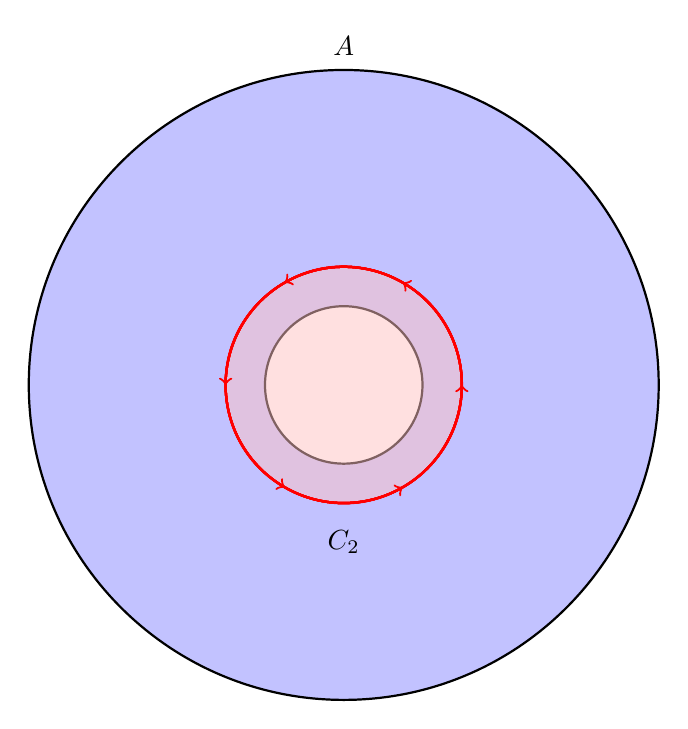
\begin{tikzpicture}
            % Define the exterior boundary
            \draw[thick, fill=blue!60!white!40] (0,0) circle (4);
        
            % Define the inner boundaries
            \draw[thick, fill=white] (0,0) circle (1);

            \draw[thick, red, fill=red!60!white!40, opacity=0.5] (0,0) circle (1.5);
            \foreach \angle in {0, 60, 120, 180, 240, 300} {
                \draw[thick, red, ->] ({1.5*cos(\angle)}, {1.5*sin(\angle)}) arc[start angle=\angle, end angle=\angle+360, radius=1.5];
            }

        
            % Label the regions
            \node at (0,4.3) {$A$};
            \node at (0,-2) {$C_2$};
            %\node at (0,1.4) {$C_0$};
        
        \end{tikzpicture}
    \end{center}
    En este caso, ya no se cumplen las condiciones del teorema de Green, puesto que $\boldsymbol{F}$ no se encuentra definida en $(0,0) \in D_2$.
    Sin embargo, es posible utilizar el teorema de Green generalizado. Definiendo previamente, con orientación positiva:
    \begin{align*}
        C_0&=\left\{(x,y): x^2+y^2=1 \right\}\\
        C_0&=\partial D_0
    \end{align*}
    \begin{center}
        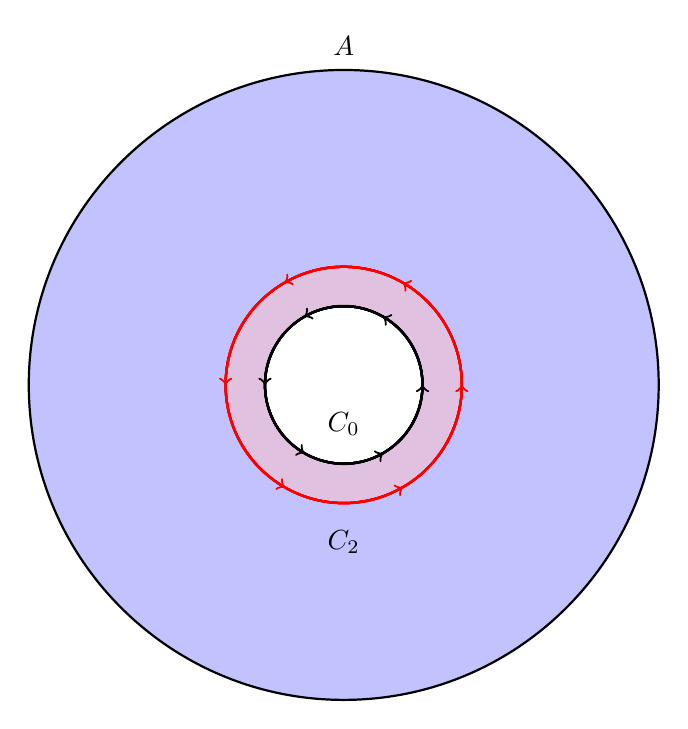
\begin{tikzpicture}
            % Define the exterior boundary
            \draw[thick, fill=blue!60!white!40] (0,0) circle (4);
        
            \draw[thick, red, fill=red!60!white!40, opacity=0.5] (0,0) circle (1.5);
            \foreach \angle in {0, 60, 120, 180, 240, 300} {
                \draw[thick, red, ->] ({1.5*cos(\angle)}, {1.5*sin(\angle)}) arc[start angle=\angle, end angle=\angle+360, radius=1.5];
            }

            % Define the inner boundaries
            \draw[thick, fill=white] (0,0) circle (1);
            \foreach \angle in {0, 60, 120, 180, 240, 300} {
                \draw[thick, ->] ({cos(\angle)}, {sin(\angle)}) arc[start angle=\angle, end angle=\angle+360, radius=1];
            }


        
            % Label the regions
            \node at (0,4.3) {$A$};
            \node at (0,-2) {$C_2$};
            \node at (0,-0.5) {$C_0$};
        
        \end{tikzpicture}
    \end{center}
    Luego, se puede utlizar el teorema de Green generalizado:
    \begin{equation*}
        \int_{C_2}\boldsymbol{F}\cdot d\boldsymbol{s} - \int_{C_0}\boldsymbol{F}\cdot d\boldsymbol{s} = \iint_{\left(D_2-D_0\right)}\left(\grad \times \boldsymbol{F}\right)dA
    \end{equation*}
    Sobre el área entre ambas curvas, el rotor del campo vale cero, puesto que está definido en $\left(D_2-D_0\right)\subset A$. Entonces, el término de la derecha, se vuelve cero.
    \begin{equation*}
        \int_{C_2}\boldsymbol{F}\cdot d\boldsymbol{s} = \int_{C_0}\boldsymbol{F}\cdot d\boldsymbol{s}
    \end{equation*}
    Para realizar la integral de la derecha, se propone la parametrización:
    \begin{equation*}
        \sigma: B=[0;2\pi] \longrightarrow \mathbb{R}^2 / \sigma(t) = (\cos(t),\sin(t))
    \end{equation*}
    \begin{equation*}
        \sigma'(t)=(-\sin(t),\cos(t))
    \end{equation*}
    Por lo tanto:
    \begin{align*}
        \int_{C_0}\boldsymbol{F}\cdot d\boldsymbol{s}&=\int_{0}^{2\pi}\boldsymbol{F}\circ\sigma(t) \cdot \sigma'(t) dt\\
        &=\int_{0}^{2\pi} (\sin(t),-\cos(t)) \cdot (-\sin(t),\cos(t)) dt\\
        &=\int_{0}^{2\pi} \left(-\sin^2(t)-\cos^2(t)\right) dt\\
        &=\int_{0}^{2\pi} -\left(\sin^2(t)+\cos^2(t)\right) dt\\
        &=-\int_{0}^{2\pi} 1 dt\\
        &=-\left.\left(t\right)\right|_{0}^{2\pi}\\
        \int_{C_0}\boldsymbol{F}\cdot d\boldsymbol{s}&=-2\pi\\
        \Rightarrow \int_{C_2}\boldsymbol{F}\cdot d\boldsymbol{s}&=-2\pi
    \end{align*}
\end{solution}

%------------Solucion 2---------------------------------------

\begin{solution}
    Primero, se debe determinar el volumen a calcular como un conjunto elemental, para poder
    realizar la integral. La primera condición del volumen, es que $x^2+y^2 \leq 9$. Luego, quedaría restringir
    en qué intervalo se encuentra el valor de $z$.
    
    Uno de los límites, como lo dice la consigna es $z=-1$.
    El otro límite es, entonces, la superficie $z=x^2+y^2$. Graficarlos nota claramente que la superficie
    descripta por el paraboloide se encuentra sobre el plano $z=-1$. Por lo tanto, la restricción para es
    $-1\leq z \leq x^2+y^2$. También se puede razonar que $0\leq x^2+y^2$ por lo que la $z=-1 < 0 \leq z=x^2+y^2$.

    Para expresar el conjunto elemental conviene hacerlo, en coordenadas cilíndricas, con $x^2+y^2=\rho^2$:
    \begin{equation*}
        \Omega = \left\{(\rho,\phi,z) \in \mathbb{R}^3 : 0\leq\rho\leq 3 \land -1\leq z \leq \rho \land 0\leq\phi\leq 2\pi \right\}
    \end{equation*}
    Ahora sí, se puede calcular el volumen en coordenadas cilíndricas:
    \begin{align*}
        \text{Vol}(\Omega)&=\iiint_\Omega dV\\
        &=\iiint_\Omega dxdydz\\
        &=\iiint_\Omega \rho d\phi dz d\rho\\
        &= \int_0^3 \int_{-1}^{\rho^2} \int_0^{2\pi} \rho d\phi dz d\rho\\
        &= \int_0^3 \int_{-1}^{\rho^2} \rho \left.\phi\right|_{\phi=0}^{\phi=2\pi} dz d\rho\\
        &= \int_0^3 \int_{-1}^{\rho^2} \rho \cdot 2\pi \cdot dz d\rho\\
        &= 2\pi \cdot \int_0^3 \rho \left.z\right|_{z=-1}^{z=\rho^2} d\rho\\
        &= 2\pi \cdot \int_0^3 \rho \left(\rho^2+1\right) d\rho\\
        &= 2\pi \cdot \int_0^3 \left(\rho^3+\rho\right) d\rho\\
        &= 2\pi \cdot \left.\left(\frac{\rho^4}{4}+\frac{\rho^2}{2}\right)\right|_{\rho=0}^{\rho=3}\\
        \therefore\text{Vol}(\Omega)&= \frac{99}{2}\pi
    \end{align*}

\end{solution}
%------------Solucion 3---------------------------------------

\begin{solution}
    Para enteder el problema, primero grafiquemos las superficies.
    \begin{center}
        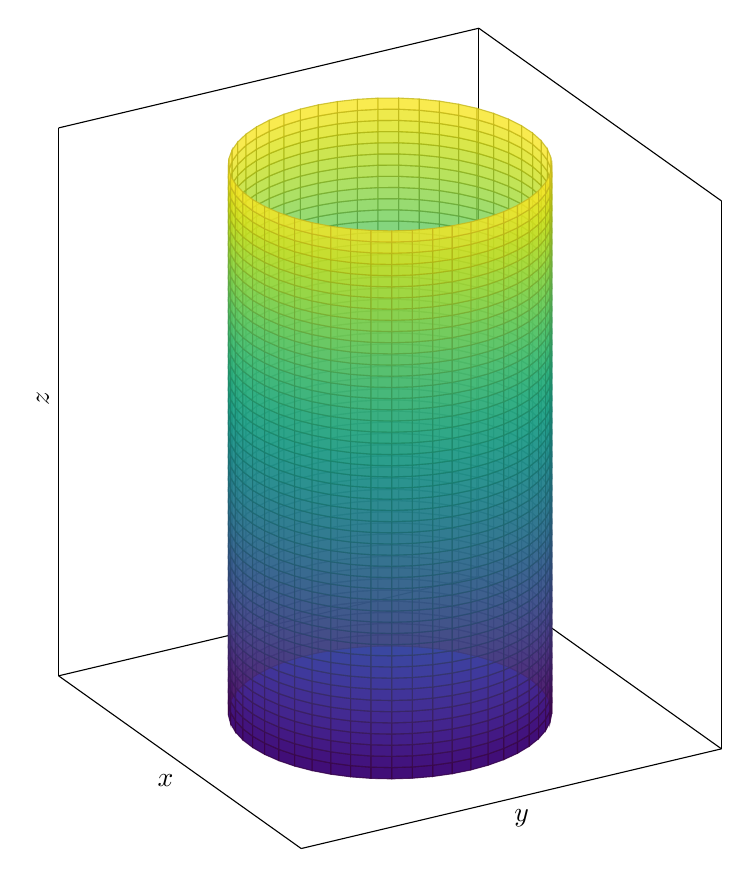
\begin{tikzpicture}
            \begin{axis}[
                    view={60}{20},
                    xlabel=$x$,
                    ylabel=$y$,
                    zlabel=$z$,
                    xmin=-1.5,
                    ymin=-1.5,
                    zmin=0,
                    xmax=1.5,
                    ymax=1.5,
                    zmax=3,
                    samples=50,
                    width=10cm,
                    height=12cm,
                    ticks=none
                ]

                \addplot3 [domain=0:360, samples=50, fill=blue, draw=none, opacity=0.8] 
                ({cos(x)}, {sin(x)}, {0});
                \addplot3 [surf, opacity=0.8, draw=none, domain=0:360, y domain=0:3, samples=50, colormap/viridis] 
                ({cos(x)}, {sin(x)}, y);   

                
            \end{axis}
        \end{tikzpicture}
    \end{center}
    Se trata de una superficie cilíndrica, con una tapa inferior en $z=0$, pero no una tapa superior en $z=3$.
    Para calcular entonces el flujo de $\boldsymbol{F}$ habría, en principio, que parametrizar la superficie cilíndrica y la
    tapa por separadas, y luego calcular dos integrales, una por cada superficie.

    Sin embargo, si se le agrega a estas dos superficies una tercera $S_T$, que sea la tapa superior del cilindro.
    Así $S_C = S_1 \bigcup S_2 \bigcup S_T$ encierra el volumen del cilindro ($\Omega$). Esta superficie $S_C = \partial\Omega$, si se
    orienta de saliente, cumple las condiciones del teorema de la divergencia. Con $\boldsymbol{F} \in \mathcal{C}^1$:
    \begin{align*}
        \iint_{S_C} \boldsymbol{F} \cdot d\boldsymbol{S} &= \iiint_{\Omega} \grad \cdot \boldsymbol{F} dV\\
        \iint_{S_1 \bigcup S_2} \boldsymbol{F} \cdot d\boldsymbol{S} + \iint_{S_T} \boldsymbol{F} \cdot d\boldsymbol{S}&= \iiint_{\Omega} \grad \cdot \boldsymbol{F} dV\\
        \iint_{S_1 \bigcup S_2} \boldsymbol{F} \cdot d\boldsymbol{S} &= \iiint_{\Omega} \grad \cdot \boldsymbol{F} dV - \iint_{S_T} \boldsymbol{F} \cdot d\boldsymbol{S}
    \end{align*}
    Ahora, se deben calcular las dos integrales del miembro derecho. Para la primera, se debe representar el $\Omega$ 
    como un conjunto elemental, lo que resulta fácil en coordenadas cilíndricas:
    \begin{equation*}
    \Omega = \left\{(\rho,\phi,z) \in \mathbb{R}^3: 0\leq\rho\leq1 \land 0\leq\phi\leq2\pi \land 0\leq z \leq 3 \right\}
    \end{equation*}
    Por lo tanto:
    \begin{align*}
        \iiint_{\Omega} \grad \cdot \boldsymbol{F} dV &= \iiint_{\Omega} \left(z-2y+x\right)dxdydz\\
        &=\iiint_{\Omega} \left(z-2\rho\sin{\phi}+\rho\cos{\phi}\right)\rho d\phi dz d\rho\\
        &=\int_{0}^{1} \int_{0}^{3} \int_{0}^{2\pi} \left(z\rho-2\rho^2\sin{\phi}+\rho^2\cos{\phi}\right) d\phi dz d\rho\\
        &= \int_{0}^{1} \int_{0}^{3}  \left.\left(z\rho\phi+2\rho^2\cos{\phi}+\rho^2\sin{\phi}\right)\right|_{\phi=0}^{\phi=2\pi} dz d\rho\\
        &= \int_{0}^{1} \int_{0}^{3}  \left(z\rho\cdot2\pi\right) dz d\rho\\
        &= \pi\int_{0}^{1}  \left.\left(z^2\rho\right)\right|_{z=0}^{z=3} d\rho\\
        &= \pi\int_{0}^{1}  \left(9\rho\right) d\rho\\
        &= 9\pi \left.\left(\frac{\rho^2}{2}\right)\right|_{\rho=0}^{\rho=1}\\
        \iiint_{\Omega} \grad \cdot \boldsymbol{F} dV&= \frac{9}{2}\pi
    \end{align*}
    Para la segunda integral a resolver, primero es necesaria la parametrización de $S_T$. Para ello, se propone 
    $D=\left\{(\rho,\phi) \in \mathbb{R}^2 : 0\leq\rho\leq1 \land 0\leq\phi\leq2\pi\right\}$ y la parametrización:
    \begin{equation*}
        \boldsymbol{\Sigma} : D \subset \mathbb{R}^2 \longrightarrow \mathbb{R}^3 / \boldsymbol{\Sigma}(\rho,\phi) = \left(\rho\cos{\phi},\rho\sin{\phi},3\right)
    \end{equation*}
    tal que $\boldsymbol{\Sigma_{\rho}}\times\boldsymbol{\Sigma_{\phi}} = \left(0,0,\rho\right)$, con $\rho>0$ orienta la superficie saliente, como se había definido previamente.
    Luego, ya es posible calcular la integral:
    \begin{align*}
        \iint_{S_T} \boldsymbol{F} \cdot d\boldsymbol{S} &= \iint_{D} (3\rho\cos{\phi},-\rho^2\sen^2{\phi},3\rho\cos{\phi}) \cdot (0,0,\rho)dA\\
        &= \iint_{D} 3\rho^2\cos{\phi}dA\\
        &= \int_{0}^{1} \int_{0}^{2\pi} 3\rho^2\cos{\phi} d\phi d\rho\\
        &= \int_{0}^{1} 3\rho^2\left.\sin{\phi}\right|_{\phi=0}^{\phi=2\pi} d\rho \\
        &= \int_{0}^{1} 3\rho^2\cdot 0 \cdot d\rho\\
        \iint_{S_T} \boldsymbol{F} \cdot d\boldsymbol{S} &= 0 \\
    \end{align*}
    Con estos dos resultados, ya es posible calcular la integral que pide la consigna, recordando que la orientación de las superficies se definió saliente.
    \begin{align*}
        \iint_{S_1 \bigcup S_2} \boldsymbol{F} \cdot d\boldsymbol{S} &= \iiint_{\Omega} \grad \cdot \boldsymbol{F} dV - \iint_{S_T} \boldsymbol{F} \cdot d\boldsymbol{S}\\
        &= \frac{9}{2}\pi - 0\\
        \therefore \iint_{S_1 \bigcup S_2} \boldsymbol{F} \cdot d\boldsymbol{S} &= \frac{9}{2}\pi
    \end{align*}
\end{solution}

%------------Solucion 4---------------------------------------

\begin{solution}
    Primero, notemos que la el campo $\boldsymbol{F}$ es un campo $\mathcal{C}^1(\mathbb{R}^3)$, puesto que
    cada una de sus componentes lo es, independientemente del valor de $a \in \mathbb{R}$.
    Por lo tanto, con $S = \partial \Omega$ orientada saliente, se cumplen las hipótesis del
    teorema de la divergencia, tal que:
    \begin{equation*}
        \iint_S \boldsymbol{F} \cdot d\boldsymbol{S} = \iiint_\Omega \grad \cdot \boldsymbol{F} dV
    \end{equation*}
    Por lo tanto, la condición que plantea la consigna:
    \begin{equation*}
        \iint_S \boldsymbol{F} \cdot d\boldsymbol{S} = \text{Vol}(\Omega)
    \end{equation*}
    se puede reescribir como:
    \begin{equation*}
        \iiint_\Omega \grad \cdot \boldsymbol{F} dV = \iiint_\Omega dV
    \end{equation*}
    Para que se cumple lo anterior, es suficiente con pedir que la divergencia del campo resulte $1$.
    \begin{align*}
        \grad \cdot \boldsymbol{F} &= 1 \\
        \partialx(ax) + \partialy(2y) + \partialz(z) &= 1 \\
        a + 2 + 1 &= 1 \\
        \therefore a &= -2
    \end{align*}
\end{solution}